% Options for packages loaded elsewhere
\PassOptionsToPackage{unicode}{hyperref}
\PassOptionsToPackage{hyphens}{url}
%
\documentclass[
]{article}
\usepackage{lmodern}
\usepackage{amssymb,amsmath}
\usepackage{ifxetex,ifluatex}
\ifnum 0\ifxetex 1\fi\ifluatex 1\fi=0 % if pdftex
  \usepackage[T1]{fontenc}
  \usepackage[utf8]{inputenc}
  \usepackage{textcomp} % provide euro and other symbols
\else % if luatex or xetex
  \usepackage{unicode-math}
  \defaultfontfeatures{Scale=MatchLowercase}
  \defaultfontfeatures[\rmfamily]{Ligatures=TeX,Scale=1}
\fi
% Use upquote if available, for straight quotes in verbatim environments
\IfFileExists{upquote.sty}{\usepackage{upquote}}{}
\IfFileExists{microtype.sty}{% use microtype if available
  \usepackage[]{microtype}
  \UseMicrotypeSet[protrusion]{basicmath} % disable protrusion for tt fonts
}{}
\makeatletter
\@ifundefined{KOMAClassName}{% if non-KOMA class
  \IfFileExists{parskip.sty}{%
    \usepackage{parskip}
  }{% else
    \setlength{\parindent}{0pt}
    \setlength{\parskip}{6pt plus 2pt minus 1pt}}
}{% if KOMA class
  \KOMAoptions{parskip=half}}
\makeatother
\usepackage{xcolor}
\IfFileExists{xurl.sty}{\usepackage{xurl}}{} % add URL line breaks if available
\IfFileExists{bookmark.sty}{\usepackage{bookmark}}{\usepackage{hyperref}}
\hypersetup{
  pdftitle={Final Project},
  pdfauthor={Sandeep Joshi},
  hidelinks,
  pdfcreator={LaTeX via pandoc}}
\urlstyle{same} % disable monospaced font for URLs
\usepackage[margin=1in]{geometry}
\usepackage{color}
\usepackage{fancyvrb}
\newcommand{\VerbBar}{|}
\newcommand{\VERB}{\Verb[commandchars=\\\{\}]}
\DefineVerbatimEnvironment{Highlighting}{Verbatim}{commandchars=\\\{\}}
% Add ',fontsize=\small' for more characters per line
\usepackage{framed}
\definecolor{shadecolor}{RGB}{248,248,248}
\newenvironment{Shaded}{\begin{snugshade}}{\end{snugshade}}
\newcommand{\AlertTok}[1]{\textcolor[rgb]{0.94,0.16,0.16}{#1}}
\newcommand{\AnnotationTok}[1]{\textcolor[rgb]{0.56,0.35,0.01}{\textbf{\textit{#1}}}}
\newcommand{\AttributeTok}[1]{\textcolor[rgb]{0.77,0.63,0.00}{#1}}
\newcommand{\BaseNTok}[1]{\textcolor[rgb]{0.00,0.00,0.81}{#1}}
\newcommand{\BuiltInTok}[1]{#1}
\newcommand{\CharTok}[1]{\textcolor[rgb]{0.31,0.60,0.02}{#1}}
\newcommand{\CommentTok}[1]{\textcolor[rgb]{0.56,0.35,0.01}{\textit{#1}}}
\newcommand{\CommentVarTok}[1]{\textcolor[rgb]{0.56,0.35,0.01}{\textbf{\textit{#1}}}}
\newcommand{\ConstantTok}[1]{\textcolor[rgb]{0.00,0.00,0.00}{#1}}
\newcommand{\ControlFlowTok}[1]{\textcolor[rgb]{0.13,0.29,0.53}{\textbf{#1}}}
\newcommand{\DataTypeTok}[1]{\textcolor[rgb]{0.13,0.29,0.53}{#1}}
\newcommand{\DecValTok}[1]{\textcolor[rgb]{0.00,0.00,0.81}{#1}}
\newcommand{\DocumentationTok}[1]{\textcolor[rgb]{0.56,0.35,0.01}{\textbf{\textit{#1}}}}
\newcommand{\ErrorTok}[1]{\textcolor[rgb]{0.64,0.00,0.00}{\textbf{#1}}}
\newcommand{\ExtensionTok}[1]{#1}
\newcommand{\FloatTok}[1]{\textcolor[rgb]{0.00,0.00,0.81}{#1}}
\newcommand{\FunctionTok}[1]{\textcolor[rgb]{0.00,0.00,0.00}{#1}}
\newcommand{\ImportTok}[1]{#1}
\newcommand{\InformationTok}[1]{\textcolor[rgb]{0.56,0.35,0.01}{\textbf{\textit{#1}}}}
\newcommand{\KeywordTok}[1]{\textcolor[rgb]{0.13,0.29,0.53}{\textbf{#1}}}
\newcommand{\NormalTok}[1]{#1}
\newcommand{\OperatorTok}[1]{\textcolor[rgb]{0.81,0.36,0.00}{\textbf{#1}}}
\newcommand{\OtherTok}[1]{\textcolor[rgb]{0.56,0.35,0.01}{#1}}
\newcommand{\PreprocessorTok}[1]{\textcolor[rgb]{0.56,0.35,0.01}{\textit{#1}}}
\newcommand{\RegionMarkerTok}[1]{#1}
\newcommand{\SpecialCharTok}[1]{\textcolor[rgb]{0.00,0.00,0.00}{#1}}
\newcommand{\SpecialStringTok}[1]{\textcolor[rgb]{0.31,0.60,0.02}{#1}}
\newcommand{\StringTok}[1]{\textcolor[rgb]{0.31,0.60,0.02}{#1}}
\newcommand{\VariableTok}[1]{\textcolor[rgb]{0.00,0.00,0.00}{#1}}
\newcommand{\VerbatimStringTok}[1]{\textcolor[rgb]{0.31,0.60,0.02}{#1}}
\newcommand{\WarningTok}[1]{\textcolor[rgb]{0.56,0.35,0.01}{\textbf{\textit{#1}}}}
\usepackage{graphicx}
\makeatletter
\def\maxwidth{\ifdim\Gin@nat@width>\linewidth\linewidth\else\Gin@nat@width\fi}
\def\maxheight{\ifdim\Gin@nat@height>\textheight\textheight\else\Gin@nat@height\fi}
\makeatother
% Scale images if necessary, so that they will not overflow the page
% margins by default, and it is still possible to overwrite the defaults
% using explicit options in \includegraphics[width, height, ...]{}
\setkeys{Gin}{width=\maxwidth,height=\maxheight,keepaspectratio}
% Set default figure placement to htbp
\makeatletter
\def\fps@figure{htbp}
\makeatother
\setlength{\emergencystretch}{3em} % prevent overfull lines
\providecommand{\tightlist}{%
  \setlength{\itemsep}{0pt}\setlength{\parskip}{0pt}}
\setcounter{secnumdepth}{-\maxdimen} % remove section numbering
\ifluatex
  \usepackage{selnolig}  % disable illegal ligatures
\fi
\newlength{\cslhangindent}
\setlength{\cslhangindent}{1.5em}
\newlength{\csllabelwidth}
\setlength{\csllabelwidth}{3em}
\newenvironment{CSLReferences}[3] % #1 hanging-ident, #2 entry sp
 {% don't indent paragraphs
  \setlength{\parindent}{0pt}
  % turn on hanging indent if param 1 is 1
  \ifodd #1 \everypar{\setlength{\hangindent}{\cslhangindent}}\ignorespaces\fi
  % set line spacing
  % set entry spacing
  \ifnum #2 > 0
  \setlength{\parskip}{#3\baselineskip}
  \fi
 }%
 {}
\usepackage{calc} % for \widthof, \maxof
\newcommand{\CSLBlock}[1]{#1\hfill\break}
\newcommand{\CSLLeftMargin}[1]{\parbox[t]{\maxof{\widthof{#1}}{\csllabelwidth}}{#1}}
\newcommand{\CSLRightInline}[1]{\parbox[t]{\linewidth}{#1}}
\newcommand{\CSLIndent}[1]{\hspace{\cslhangindent}#1}

\title{Final Project}
\author{Sandeep Joshi}
\date{2020-12-15}

\begin{document}
\maketitle

\hypertarget{introduction}{%
\subsubsection{Introduction}\label{introduction}}

This study explores sentiments driven through Tweets of famous people
and the contexts related to these sentiments. As observed during recent
Presidential elections of the United States and often heard in political
commentary, public opinion remains divisive and it seems to be ever
increasing with social media platforms becoming the progenitor and
proliferator of this divide.

Social media platforms like Twitter, Facebook, Google search, etc. wield
an ever-increasing influence on our society and its opinions. Numerous
recent congressional hearings over antitrust and election meddling
involving such platforms would be a testament to that influence.
Everyday numerous political hashtags emerge, a few of which snowball
into big political movements.

As potent as these platforms are, they are often rife with fake news and
propogandas. Coupled with behaviourally- conditioned, AI-driven news
aggregation and streaming, they wield strong clout in forming and
guiding public opinions towards extremes.

Numerous studies over the years like A. and Sonawane (2016) and Davidov,
Tsur, and Rappoport (2010) have employed techniques of Natural language
processing (NLP) and Machine Learning (ML). To solve the problem of
analyzing sentiment in a small text of a tweet. Davidov, Tsur, and
Rappoport (2010) had employed and built upon numerous techniques based
off of earlier works and provided a comparative analysis of popular ML
techniques like Naive Bayes, Bi-grams, Support Vector Machines.

Almost all of the studies I have reviewed, followed a popular hashtag or
Tweets of a user over a large period of time to have sizable data
sufficient for analysis. This study however, employs many of these well
established methods, over a singular context to explore how a tweet is
perceived by different sections of society and how these different
perceptions may drive different opinions.

Techniques and models developed in this endeavor could be used for
further research on the topic of social influences with different
themes. Social feedback on any policies, approval ratings of sitting
president to Big brother next vote out. Such models could also be used
to prioritizing fact checking tweets which rank higher on say certain
topics or having more polarizing effects in communities.

\hypertarget{research-question}{%
\subsubsection{Research Question}\label{research-question}}

The primary objective of this study is to explore the different
sentiments driven by President Trump over Twitter and try to understand
these affects within the tweets' political or social context. The study
explores the responses on President Trump's tweets and tries to
understand if these replies exhibit any polarization or factions.

President Trump:

\begin{quote}
``My use of social media is not Presidential - it's MODERN DAY
PRESIDENTIAL. Make America Great Again!''
\end{quote}

\raggedleft

-- President Donald Trump (via twitter @realDonaldTrump).

\hypertarget{method}{%
\subsubsection{Method}\label{method}}

\hypertarget{data}{%
\paragraph{Data}\label{data}}

President Donald Trump is perhaps the most prolific tweeters among
modern-day world leaders. In his fourth year, he averages staggering
33.2 tweets per day\footnote{\url{http://www.trumptwitterarchive.com/archive}}!
He has tweeted over 51,000 times over the last five years\footnote{\url{https://www.trackalytics.com/twitter/profile/realdonaldtrump/}}.
He has truly embraced social media like no other leader before or
present.

Expectedly, because of his post as one of the most influential leaders
in the world and his prolific usage of twitter, his tweets have already
been a topic of numerous studies and articles. A slew of such articles -
Keown (2020) and Liu (2020) and papers like Kleczka (2020) and Ge,
Kurov, and Wolfe (2018) became motivation towards this study.

This study employs Twitter's fresh off the oven API v2 to download
recent President's Trumps' tweet from his personal handle
@realDonaldTrump, other twitter metadata like - likes, retweets, quotes
and the replies of other users on the tweet. Most of his recent tweets
are regarding results of the presidential election, claims of the voter
fraud and possible recounting of votes. All these tweets have triggered
contrasting responses from Republicans and democrats alike and many of
these choses to flock to the president's twitter handle to denote their
opinions on his posts.

A separate python
\href{https://github.com/Sandeep-Joshi/twitter_api/blob/main/TwitterUsers.py}{script}
was used to scrape this data and create a csv files for President's
tweets and another csv file type to store different reply threads.

Some of the tweets had over 80k replies!

\hypertarget{approach}{%
\paragraph{Approach}\label{approach}}

\begin{enumerate}
\def\labelenumi{\arabic{enumi}.}
\tightlist
\item
  My study would employ the Syuzhet package in R for sentiment analysis
  and classification of the replies.
\item
  It would then employ cluster analysis to break the sentiment space
  into two clusters - one who supports/ agrees with President Trump and
  a cluster who doesn't.
\item
  I would then explore the positivity and negativity associated with
  these clusters.
\item
  And lastly, I would perform topic modelling to understand the context
  of these sentiments.
\end{enumerate}

\hypertarget{procedure}{%
\subsubsection{Procedure}\label{procedure}}

\hypertarget{load-data-scraped-in-python-in-r}{%
\paragraph{Load Data scraped in python in
R}\label{load-data-scraped-in-python-in-r}}

\begin{Shaded}
\begin{Highlighting}[]
\NormalTok{replies\_index }\OtherTok{=} \FunctionTok{list.files}\NormalTok{(}\StringTok{\textquotesingle{}replies\textquotesingle{}}\NormalTok{)}

\CommentTok{\# load tweet and its replies.}
\NormalTok{tweets\_df }\OtherTok{\textless{}{-}}  \FunctionTok{read.csv2}\NormalTok{(}\StringTok{\textquotesingle{}Practice Tweets.csv\textquotesingle{}}\NormalTok{, }\AttributeTok{stringsAsFactors=}\ConstantTok{FALSE}\NormalTok{, }\AttributeTok{sep =} \StringTok{\textquotesingle{},\textquotesingle{}}\NormalTok{, }\AttributeTok{numerals =} \FunctionTok{c}\NormalTok{(}\StringTok{"no.loss"}\NormalTok{))}
\NormalTok{tweets\_df[,}\FunctionTok{c}\NormalTok{(}\StringTok{\textquotesingle{}ID\textquotesingle{}}\NormalTok{)] }\OtherTok{\textless{}{-}} \FunctionTok{sapply}\NormalTok{(tweets\_df[,}\FunctionTok{c}\NormalTok{(}\StringTok{\textquotesingle{}ID\textquotesingle{}}\NormalTok{)], as.String)}
\NormalTok{tweets\_df}\SpecialCharTok{$}\NormalTok{Topic\_terms\_2 }\OtherTok{=}\NormalTok{ tweets\_df}\SpecialCharTok{$}\NormalTok{Topic\_terms\_1 }\OtherTok{=} \StringTok{\textquotesingle{}\textquotesingle{}}  \CommentTok{\# instantiate new column for storing Topic models}
\end{Highlighting}
\end{Shaded}

\hypertarget{clean-data}{%
\paragraph{Clean Data}\label{clean-data}}

\begin{Shaded}
\begin{Highlighting}[]
\CommentTok{\# Clean tweets}
\NormalTok{clean\_replies }\OtherTok{\textless{}{-}} \ControlFlowTok{function}\NormalTok{(reply) \{}
\NormalTok{  clean\_tweet }\OtherTok{\textless{}{-}} \FunctionTok{str\_remove\_all}\NormalTok{(reply, }\StringTok{"@.*?(}\SpecialCharTok{\textbackslash{}\textbackslash{}}\StringTok{s+?|$)|\^{}RT |http.*?(}\SpecialCharTok{\textbackslash{}\textbackslash{}}\StringTok{s+?|$)"}\NormalTok{) }\CommentTok{\# To remove @twitter handles and Retweet tag.}
\NormalTok{  clean\_tweet }\OtherTok{\textless{}{-}} \FunctionTok{tolower}\NormalTok{(clean\_tweet)}
\NormalTok{  clean\_tweet }\OtherTok{\textless{}{-}} \FunctionTok{str\_squish}\NormalTok{(}\FunctionTok{str\_trim}\NormalTok{(clean\_tweet))}
  \CommentTok{\# Not removing punctuations as some libraries use emoticons to analyze tweets}
\NormalTok{  clean\_tweet }\OtherTok{\textless{}{-}} \FunctionTok{removeWords}\NormalTok{(clean\_tweet, }\FunctionTok{stopwords}\NormalTok{(}\StringTok{\textquotesingle{}en\textquotesingle{}}\NormalTok{)) }\CommentTok{\# delete stopwords from text}
\NormalTok{  clean\_tweet }\OtherTok{\textless{}{-}} \FunctionTok{stem\_strings}\NormalTok{(clean\_tweet) }\CommentTok{\# stemming. Might need to remove it as it can confuse certain sentiment analyses}
  \FunctionTok{return}\NormalTok{(clean\_tweet)}
\NormalTok{\}}
\end{Highlighting}
\end{Shaded}

\hypertarget{check-if-we-have-reply-data-for-the-tweet}{%
\paragraph{Check if we have reply data for the
Tweet}\label{check-if-we-have-reply-data-for-the-tweet}}

\begin{Shaded}
\begin{Highlighting}[]
\CommentTok{\# Check if we have replies data for the tweet using conversation id}
\NormalTok{check\_replies }\OtherTok{\textless{}{-}} \ControlFlowTok{function}\NormalTok{(tweet) \{}
\NormalTok{  reply\_file }\OtherTok{=} \FunctionTok{paste0}\NormalTok{(tweet[,}\DecValTok{3}\NormalTok{], }\StringTok{".csv"}\NormalTok{)}
  \ControlFlowTok{if}\NormalTok{ (reply\_file }\SpecialCharTok{\%in\%}\NormalTok{ replies\_index)\{}
    \CommentTok{\# reply found, work with tweet}
    \FunctionTok{cat}\NormalTok{(}\StringTok{"Tweet: "}\NormalTok{, tweet[,}\DecValTok{8}\NormalTok{], }\StringTok{" "}\NormalTok{)}
    \FunctionTok{cat}\NormalTok{(}\StringTok{"Likes: "}\NormalTok{, tweet[,}\DecValTok{7}\NormalTok{], }\StringTok{"and Retweets: "}\NormalTok{, tweet[,}\DecValTok{6}\NormalTok{], }\StringTok{". "}\NormalTok{)}
\NormalTok{    reply\_file }\OtherTok{\textless{}{-}} \FunctionTok{paste0}\NormalTok{(}\StringTok{\textquotesingle{}replies/\textquotesingle{}}\NormalTok{, reply\_file)}
    \FunctionTok{cat}\NormalTok{(}\StringTok{"Found replies file: "}\NormalTok{, reply\_file)}
\NormalTok{    reply\_df }\OtherTok{\textless{}{-}} \FunctionTok{read.csv}\NormalTok{(reply\_file)}
    \FunctionTok{cat}\NormalTok{(}\StringTok{"Number of replies found: "}\NormalTok{, }\FunctionTok{nrow}\NormalTok{(reply\_df), }\StringTok{". }\SpecialCharTok{\textbackslash{}n}\StringTok{"}\NormalTok{)}
\NormalTok{    reply\_df}\SpecialCharTok{$}\NormalTok{Text }\OtherTok{\textless{}{-}} \FunctionTok{lapply}\NormalTok{(reply\_df}\SpecialCharTok{$}\NormalTok{Text, clean\_replies)}
    \FunctionTok{return}\NormalTok{(reply\_df)}
\NormalTok{  \} }
  \ControlFlowTok{else}\NormalTok{ \{}
    \FunctionTok{return}\NormalTok{(}\ConstantTok{NULL}\NormalTok{)}
\NormalTok{  \}}
\NormalTok{\}}
\end{Highlighting}
\end{Shaded}

\hypertarget{running-sentiment-analysis-on-tweets}{%
\paragraph{Running sentiment analysis on
tweets}\label{running-sentiment-analysis-on-tweets}}

\begin{Shaded}
\begin{Highlighting}[]
\NormalTok{sentiment\_score }\OtherTok{\textless{}{-}} \ControlFlowTok{function}\NormalTok{(tweet) \{}
  \CommentTok{\# Syuzhet. Other methods are “bing”, “afinn”, “nrc”, and “stanford”}
  \CommentTok{\# browser()}
  \FunctionTok{return}\NormalTok{(}\FunctionTok{get\_nrc\_sentiment}\NormalTok{(tweet))}
\NormalTok{\}}

\CommentTok{\# Topic modeling on tweets to 2 topics}
\NormalTok{topic\_model }\OtherTok{\textless{}{-}} \ControlFlowTok{function}\NormalTok{(tweet\_col) \{}
\NormalTok{  reply\_corpus }\OtherTok{\textless{}{-}} \FunctionTok{Corpus}\NormalTok{(}\FunctionTok{VectorSource}\NormalTok{(tweet\_col))}
  \CommentTok{\# Stemming, stop words have been taken care of earlier}
\NormalTok{  import\_mat }\OtherTok{\textless{}{-}} \FunctionTok{DocumentTermMatrix}\NormalTok{(reply\_corpus, }\AttributeTok{control =} \FunctionTok{list}\NormalTok{(}\AttributeTok{stemming =}\ConstantTok{TRUE}\NormalTok{,}
                                                                \AttributeTok{stopwords =} \ConstantTok{TRUE}\NormalTok{,}
                                                                \AttributeTok{minWordLength =} \DecValTok{3}\NormalTok{, }\CommentTok{\# This keeps the data out of sync}
                                                                \AttributeTok{removeNumbers =} \ConstantTok{TRUE}\NormalTok{,}
                                                                \AttributeTok{removePunctuation =}\ConstantTok{TRUE}\NormalTok{))}
\NormalTok{  import\_weight }\OtherTok{=} \FunctionTok{tapply}\NormalTok{(import\_mat}\SpecialCharTok{$}\NormalTok{v}\SpecialCharTok{/}\FunctionTok{row\_sums}\NormalTok{(import\_mat)[import\_mat}\SpecialCharTok{$}\NormalTok{i], }
\NormalTok{                       import\_mat}\SpecialCharTok{$}\NormalTok{j, }
\NormalTok{                       mean) }\SpecialCharTok{*}
    \FunctionTok{log2}\NormalTok{(}\FunctionTok{nDocs}\NormalTok{(import\_mat)}\SpecialCharTok{/}\FunctionTok{col\_sums}\NormalTok{(import\_mat }\SpecialCharTok{\textgreater{}} \DecValTok{0}\NormalTok{))}
  
  \CommentTok{\#ignore very frequent and 0 terms}
\NormalTok{  import\_mat }\OtherTok{=}\NormalTok{ import\_mat[ }\FunctionTok{row\_sums}\NormalTok{(import\_mat) }\SpecialCharTok{\textgreater{}} \DecValTok{0}\NormalTok{, ]}
  
  \CommentTok{\# 2 topics and random seed of 7}
\NormalTok{  LDA\_gibbs }\OtherTok{=} \FunctionTok{LDA}\NormalTok{(import\_mat, }\AttributeTok{k =} \DecValTok{2}\NormalTok{, }\AttributeTok{method =} \StringTok{"Gibbs"}\NormalTok{, }
                \AttributeTok{control =} \FunctionTok{list}\NormalTok{(}\AttributeTok{seed =} \DecValTok{7}\NormalTok{, }\AttributeTok{burnin =} \DecValTok{1000}\NormalTok{, }
                               \AttributeTok{thin =} \DecValTok{100}\NormalTok{, }\AttributeTok{iter =} \DecValTok{1000}\NormalTok{))}
  \CommentTok{\# See Topic modelings values to verify all indicators are within control and expected range}
  \FunctionTok{cat}\NormalTok{(}\StringTok{"LDA Gibb\textquotesingle{}s Alpha: "}\NormalTok{, LDA\_gibbs}\SpecialCharTok{@}\NormalTok{alpha, }
      \StringTok{"entropy: "}\NormalTok{, }\FunctionTok{mean}\NormalTok{(}\FunctionTok{apply}\NormalTok{(}\FunctionTok{posterior}\NormalTok{(LDA\_gibbs)}\SpecialCharTok{$}\NormalTok{topics, }\DecValTok{1}\NormalTok{, }\ControlFlowTok{function}\NormalTok{(z) }\SpecialCharTok{{-}} \FunctionTok{sum}\NormalTok{(z }\SpecialCharTok{*} \FunctionTok{log}\NormalTok{(z)))))}
  
  \CommentTok{\# Return lists from models so that they can be added to df. Complete model doesn\textquotesingle{}t work}
  \FunctionTok{return}\NormalTok{(}\FunctionTok{list}\NormalTok{(}\StringTok{"topics"} \OtherTok{=} \FunctionTok{tidy}\NormalTok{(LDA\_gibbs, }\AttributeTok{matrix =} \StringTok{"gamma"}\NormalTok{), }\StringTok{"terms"} \OtherTok{=} \FunctionTok{terms}\NormalTok{(LDA\_gibbs, }\DecValTok{20}\NormalTok{)))}
\NormalTok{\}}
\end{Highlighting}
\end{Shaded}

\hypertarget{topic-modelling-over-entire-corpus-of-replies-on-a-single-tweet.}{%
\paragraph{Topic modelling over entire corpus of replies on a single
tweet.}\label{topic-modelling-over-entire-corpus-of-replies-on-a-single-tweet.}}

\begin{Shaded}
\begin{Highlighting}[]
\NormalTok{get\_all\_modeling\_data }\OtherTok{\textless{}{-}} \ControlFlowTok{function}\NormalTok{(tweet\_id) \{}
    
    \FunctionTok{sprintf}\NormalTok{(}\StringTok{"For tweet id: \%s "}\NormalTok{, tweet\_id)}
\NormalTok{    replies }\OtherTok{=} \FunctionTok{check\_replies}\NormalTok{(tweets\_df[tweets\_df}\SpecialCharTok{$}\NormalTok{ID }\SpecialCharTok{==}\NormalTok{ tweet\_id,])}
    \CommentTok{\# Delete blank replies as this causes issues later on with DF operations.}
\NormalTok{    replies }\OtherTok{\textless{}{-}}\NormalTok{ replies[}\SpecialCharTok{!}\FunctionTok{grepl}\NormalTok{(}\StringTok{"\^{}}\SpecialCharTok{\textbackslash{}\textbackslash{}}\StringTok{s*$"}\NormalTok{,replies}\SpecialCharTok{$}\NormalTok{Text),]}
    
    \ControlFlowTok{if}\NormalTok{ (}\SpecialCharTok{!}\FunctionTok{is.null}\NormalTok{(replies)) \{}
\NormalTok{      replies}\SpecialCharTok{$}\NormalTok{Topic\_category }\OtherTok{\textless{}{-}} \DecValTok{0}
      \CommentTok{\# Do sentiment analysis for each reply}
\NormalTok{      replies }\OtherTok{\textless{}{-}} \FunctionTok{cbind}\NormalTok{(replies, }\FunctionTok{bind\_rows}\NormalTok{(}\FunctionTok{lapply}\NormalTok{(replies}\SpecialCharTok{$}\NormalTok{Text, sentiment\_score)))}
      \FunctionTok{sprintf}\NormalTok{(}\StringTok{"Sentiment analysis done for all replies on Tweet \%s}\SpecialCharTok{\textbackslash{}n}\StringTok{"}\NormalTok{, tweet\_id)}
      
      \CommentTok{\# Do Topic modeling for all replies.}
\NormalTok{      temp\_model }\OtherTok{\textless{}{-}} \FunctionTok{topic\_model}\NormalTok{(replies}\SpecialCharTok{$}\NormalTok{Text)  }
      
      \CommentTok{\# Add top terms in all replies corpus to Tweet data}
\NormalTok{      Topic\_terms\_1 }\OtherTok{\textless{}{-}} \FunctionTok{toString}\NormalTok{(temp\_model}\SpecialCharTok{$}\NormalTok{terms[,}\DecValTok{1}\NormalTok{])}
\NormalTok{      Topic\_terms\_2 }\OtherTok{\textless{}{-}} \FunctionTok{toString}\NormalTok{(temp\_model}\SpecialCharTok{$}\NormalTok{terms[,}\DecValTok{2}\NormalTok{])}

      
      \CommentTok{\# Add Topic category to the reply, determined by highest beta value. Equal values are not classified.}
\NormalTok{      temp\_topics }\OtherTok{\textless{}{-}}\NormalTok{ temp\_model}\SpecialCharTok{$}\NormalTok{topics }\SpecialCharTok{\%\textgreater{}\%} \FunctionTok{group\_by}\NormalTok{(document) }\SpecialCharTok{\%\textgreater{}\%} 
        \FunctionTok{filter}\NormalTok{(gamma}\SpecialCharTok{==}\FunctionTok{max}\NormalTok{(gamma)) }\SpecialCharTok{\%\textgreater{}\%} 
        \FunctionTok{arrange}\NormalTok{(document, topic)}
\NormalTok{      temp\_topics }\OtherTok{\textless{}{-}}\NormalTok{ temp\_topics }\SpecialCharTok{\%\textgreater{}\%} \FunctionTok{filter}\NormalTok{(gamma }\SpecialCharTok{!=} \FloatTok{0.5000000}\NormalTok{) }\SpecialCharTok{\%\textgreater{}\%} \FunctionTok{select}\NormalTok{(document, topic)}
      
      \ControlFlowTok{for}\NormalTok{ (j }\ControlFlowTok{in} \DecValTok{1}\SpecialCharTok{:}\FunctionTok{nrow}\NormalTok{(replies)) \{}
\NormalTok{        replies[j,]}\SpecialCharTok{$}\NormalTok{Topic\_category }\OtherTok{\textless{}{-}} \FunctionTok{toString}\NormalTok{(temp\_topics[temp\_topics}\SpecialCharTok{$}\NormalTok{document}\SpecialCharTok{==}\FunctionTok{toString}\NormalTok{(j),]}\SpecialCharTok{$}\NormalTok{topic)}
\NormalTok{      \}}
      
      \CommentTok{\# remove temp\_model from memory to save space}
      \FunctionTok{rm}\NormalTok{(}\AttributeTok{list=}\FunctionTok{c}\NormalTok{(}\StringTok{\textquotesingle{}temp\_model\textquotesingle{}}\NormalTok{, }\StringTok{\textquotesingle{}temp\_topics\textquotesingle{}}\NormalTok{))}
      
      \FunctionTok{sprintf}\NormalTok{(}\StringTok{"Topic Modelling done for Tweet \%s"}\NormalTok{, tweet\_id)}
      \FunctionTok{return}\NormalTok{(}\FunctionTok{list}\NormalTok{(}\StringTok{"replies"}\OtherTok{=}\NormalTok{replies, }\StringTok{"topic\_terms1"}\OtherTok{=}\NormalTok{Topic\_terms\_1, }\StringTok{"topic\_terms2"}\OtherTok{=}\NormalTok{Topic\_terms\_2))}
\NormalTok{    \}}
\NormalTok{\}}
\end{Highlighting}
\end{Shaded}

\hypertarget{running-my-model-on-presidential-tweets-between-dec-07th-and-dec-08th-2020}{%
\paragraph{Running my model on Presidential Tweets between Dec 07th and
Dec 08th
2020}\label{running-my-model-on-presidential-tweets-between-dec-07th-and-dec-08th-2020}}

\begin{Shaded}
\begin{Highlighting}[]
\CommentTok{\# Tweet: 1335775535717289984}
\NormalTok{tweet\_id }\OtherTok{=} \StringTok{\textquotesingle{}1335775535717289984\textquotesingle{}}
\NormalTok{temp\_reply }\OtherTok{\textless{}{-}} \FunctionTok{get\_all\_modeling\_data}\NormalTok{(tweet\_id)}
\NormalTok{reply\_model\_1335775535717289984 }\OtherTok{\textless{}{-}}\NormalTok{ temp\_reply}\SpecialCharTok{$}\NormalTok{replies}
\NormalTok{tweets\_df[tweets\_df}\SpecialCharTok{$}\NormalTok{ID }\SpecialCharTok{==}\NormalTok{ tweet\_id,]}\SpecialCharTok{$}\NormalTok{Topic\_terms\_1 }\OtherTok{\textless{}{-}} \FunctionTok{toString}\NormalTok{(temp\_reply}\SpecialCharTok{$}\NormalTok{topic\_terms1)}
\NormalTok{tweets\_df[tweets\_df}\SpecialCharTok{$}\NormalTok{ID }\SpecialCharTok{==}\NormalTok{ tweet\_id,]}\SpecialCharTok{$}\NormalTok{Topic\_terms\_2 }\OtherTok{\textless{}{-}} \FunctionTok{toString}\NormalTok{(temp\_reply}\SpecialCharTok{$}\NormalTok{topic\_terms2)}


\CommentTok{\# Tweet: 1335971721262796801}
\NormalTok{tweet\_id }\OtherTok{=} \StringTok{\textquotesingle{}1335971721262796801\textquotesingle{}}
\NormalTok{temp\_reply }\OtherTok{\textless{}{-}} \FunctionTok{get\_all\_modeling\_data}\NormalTok{(tweet\_id)}
\NormalTok{reply\_model\_1335971721262796801 }\OtherTok{\textless{}{-}}\NormalTok{ temp\_reply}\SpecialCharTok{$}\NormalTok{replies}
\NormalTok{tweets\_df[tweets\_df}\SpecialCharTok{$}\NormalTok{ID }\SpecialCharTok{==}\NormalTok{ tweet\_id,]}\SpecialCharTok{$}\NormalTok{Topic\_terms\_1 }\OtherTok{\textless{}{-}} \FunctionTok{toString}\NormalTok{(temp\_reply}\SpecialCharTok{$}\NormalTok{topic\_terms1)}
\NormalTok{tweets\_df[tweets\_df}\SpecialCharTok{$}\NormalTok{ID }\SpecialCharTok{==}\NormalTok{ tweet\_id,]}\SpecialCharTok{$}\NormalTok{Topic\_terms\_2 }\OtherTok{\textless{}{-}} \FunctionTok{toString}\NormalTok{(temp\_reply}\SpecialCharTok{$}\NormalTok{topic\_terms2)}

\CommentTok{\# Tweet: 1335984976521801733}
\NormalTok{tweet\_id }\OtherTok{=} \StringTok{\textquotesingle{}1335984976521801733\textquotesingle{}}
\NormalTok{temp\_reply }\OtherTok{\textless{}{-}} \FunctionTok{get\_all\_modeling\_data}\NormalTok{(tweet\_id)}
\NormalTok{reply\_model\_1335984976521801733 }\OtherTok{\textless{}{-}}\NormalTok{ temp\_reply}\SpecialCharTok{$}\NormalTok{replies}
\NormalTok{tweets\_df[tweets\_df}\SpecialCharTok{$}\NormalTok{ID }\SpecialCharTok{==}\NormalTok{ tweet\_id,]}\SpecialCharTok{$}\NormalTok{Topic\_terms\_1 }\OtherTok{\textless{}{-}} \FunctionTok{toString}\NormalTok{(temp\_reply}\SpecialCharTok{$}\NormalTok{topic\_terms1)}
\NormalTok{tweets\_df[tweets\_df}\SpecialCharTok{$}\NormalTok{ID }\SpecialCharTok{==}\NormalTok{ tweet\_id,]}\SpecialCharTok{$}\NormalTok{Topic\_terms\_2 }\OtherTok{\textless{}{-}} \FunctionTok{toString}\NormalTok{(temp\_reply}\SpecialCharTok{$}\NormalTok{topic\_terms2)}

\CommentTok{\# Tweet: 1336148836495069185}
\NormalTok{tweet\_id }\OtherTok{=} \StringTok{\textquotesingle{}1336148836495069185\textquotesingle{}}
\NormalTok{temp\_reply }\OtherTok{\textless{}{-}} \FunctionTok{get\_all\_modeling\_data}\NormalTok{(tweet\_id)}
\NormalTok{reply\_model\_1336148836495069185 }\OtherTok{\textless{}{-}}\NormalTok{ temp\_reply}\SpecialCharTok{$}\NormalTok{replies}
\NormalTok{tweets\_df[tweets\_df}\SpecialCharTok{$}\NormalTok{ID }\SpecialCharTok{==}\NormalTok{ tweet\_id,]}\SpecialCharTok{$}\NormalTok{Topic\_terms\_1 }\OtherTok{\textless{}{-}} \FunctionTok{toString}\NormalTok{(temp\_reply}\SpecialCharTok{$}\NormalTok{topic\_terms1)}
\NormalTok{tweets\_df[tweets\_df}\SpecialCharTok{$}\NormalTok{ID }\SpecialCharTok{==}\NormalTok{ tweet\_id,]}\SpecialCharTok{$}\NormalTok{Topic\_terms\_2 }\OtherTok{\textless{}{-}} \FunctionTok{toString}\NormalTok{(temp\_reply}\SpecialCharTok{$}\NormalTok{topic\_terms2)}

\CommentTok{\# Tweet: 1336318760106471424}
\NormalTok{tweet\_id }\OtherTok{=} \StringTok{\textquotesingle{}1336318760106471424\textquotesingle{}}
\NormalTok{temp\_reply }\OtherTok{\textless{}{-}} \FunctionTok{get\_all\_modeling\_data}\NormalTok{(tweet\_id)}
\NormalTok{reply\_model\_1336318760106471424 }\OtherTok{\textless{}{-}}\NormalTok{ temp\_reply}\SpecialCharTok{$}\NormalTok{replies}
\NormalTok{tweets\_df[tweets\_df}\SpecialCharTok{$}\NormalTok{ID }\SpecialCharTok{==}\NormalTok{ tweet\_id,]}\SpecialCharTok{$}\NormalTok{Topic\_terms\_1 }\OtherTok{\textless{}{-}} \FunctionTok{toString}\NormalTok{(temp\_reply}\SpecialCharTok{$}\NormalTok{topic\_terms1)}
\NormalTok{tweets\_df[tweets\_df}\SpecialCharTok{$}\NormalTok{ID }\SpecialCharTok{==}\NormalTok{ tweet\_id,]}\SpecialCharTok{$}\NormalTok{Topic\_terms\_2 }\OtherTok{\textless{}{-}} \FunctionTok{toString}\NormalTok{(temp\_reply}\SpecialCharTok{$}\NormalTok{topic\_terms2)}

\CommentTok{\# Tweet: 1336110929856040960}
\NormalTok{tweet\_id }\OtherTok{=} \StringTok{\textquotesingle{}1336110929856040960\textquotesingle{}}
\NormalTok{temp\_reply }\OtherTok{\textless{}{-}} \FunctionTok{get\_all\_modeling\_data}\NormalTok{(tweet\_id)}
\NormalTok{reply\_model\_1336110929856040960 }\OtherTok{\textless{}{-}}\NormalTok{ temp\_reply}\SpecialCharTok{$}\NormalTok{replies}
\NormalTok{tweets\_df[tweets\_df}\SpecialCharTok{$}\NormalTok{ID }\SpecialCharTok{==}\NormalTok{ tweet\_id,]}\SpecialCharTok{$}\NormalTok{Topic\_terms\_1 }\OtherTok{\textless{}{-}} \FunctionTok{toString}\NormalTok{(temp\_reply}\SpecialCharTok{$}\NormalTok{topic\_terms1)}
\NormalTok{tweets\_df[tweets\_df}\SpecialCharTok{$}\NormalTok{ID }\SpecialCharTok{==}\NormalTok{ tweet\_id,]}\SpecialCharTok{$}\NormalTok{Topic\_terms\_2 }\OtherTok{\textless{}{-}} \FunctionTok{toString}\NormalTok{(temp\_reply}\SpecialCharTok{$}\NormalTok{topic\_terms2)}


\CommentTok{\# Tweet: 1336112582424473600}
\NormalTok{tweet\_id }\OtherTok{=} \StringTok{\textquotesingle{}1336112582424473600\textquotesingle{}}
\NormalTok{temp\_reply }\OtherTok{\textless{}{-}} \FunctionTok{get\_all\_modeling\_data}\NormalTok{(tweet\_id)}
\NormalTok{reply\_model\_1336112582424473600 }\OtherTok{\textless{}{-}}\NormalTok{ temp\_reply}\SpecialCharTok{$}\NormalTok{replies}
\NormalTok{tweets\_df[tweets\_df}\SpecialCharTok{$}\NormalTok{ID }\SpecialCharTok{==}\NormalTok{ tweet\_id,]}\SpecialCharTok{$}\NormalTok{Topic\_terms\_1 }\OtherTok{\textless{}{-}} \FunctionTok{toString}\NormalTok{(temp\_reply}\SpecialCharTok{$}\NormalTok{topic\_terms1)}
\NormalTok{tweets\_df[tweets\_df}\SpecialCharTok{$}\NormalTok{ID }\SpecialCharTok{==}\NormalTok{ tweet\_id,]}\SpecialCharTok{$}\NormalTok{Topic\_terms\_2 }\OtherTok{\textless{}{-}} \FunctionTok{toString}\NormalTok{(temp\_reply}\SpecialCharTok{$}\NormalTok{topic\_terms2)}
\end{Highlighting}
\end{Shaded}

\hypertarget{calculate-sentiment-metadata-for-tweet}{%
\paragraph{Calculate sentiment metadata for
Tweet}\label{calculate-sentiment-metadata-for-tweet}}

\begin{Shaded}
\begin{Highlighting}[]
\NormalTok{tweet\_ids }\OtherTok{\textless{}{-}} \FunctionTok{c}\NormalTok{(}\StringTok{\textquotesingle{}1335775535717289984\textquotesingle{}}\NormalTok{, }\StringTok{\textquotesingle{}1335971721262796801\textquotesingle{}}\NormalTok{, }\StringTok{\textquotesingle{}1335984976521801733\textquotesingle{}}\NormalTok{, }\StringTok{\textquotesingle{}1336148836495069185\textquotesingle{}}\NormalTok{, }\StringTok{\textquotesingle{}1336318760106471424\textquotesingle{}}\NormalTok{, }\StringTok{\textquotesingle{}1336110929856040960\textquotesingle{}}\NormalTok{, }\StringTok{\textquotesingle{}1336112582424473600\textquotesingle{}}\NormalTok{)}
\NormalTok{meta\_cols }\OtherTok{\textless{}{-}} \FunctionTok{c}\NormalTok{(}\StringTok{\textquotesingle{}anger\textquotesingle{}}\NormalTok{, }\StringTok{\textquotesingle{}anticipation\textquotesingle{}}\NormalTok{, }\StringTok{\textquotesingle{}disgust\textquotesingle{}}\NormalTok{,}\StringTok{\textquotesingle{}fear\textquotesingle{}}\NormalTok{,}\StringTok{\textquotesingle{}joy\textquotesingle{}}\NormalTok{,}\StringTok{\textquotesingle{}sadness\textquotesingle{}}\NormalTok{,}\StringTok{\textquotesingle{}surprise\textquotesingle{}}\NormalTok{,}\StringTok{\textquotesingle{}trust\textquotesingle{}}\NormalTok{,}\StringTok{\textquotesingle{}positive\textquotesingle{}}\NormalTok{,}\StringTok{\textquotesingle{}negative\textquotesingle{}}\NormalTok{)}


\NormalTok{replies\_metadata\_df }\OtherTok{\textless{}{-}} \FunctionTok{data.frame}\NormalTok{(}\AttributeTok{row.names =} \FunctionTok{c}\NormalTok{(}\StringTok{\textquotesingle{}id\textquotesingle{}}\NormalTok{, meta\_cols))}

\ControlFlowTok{for}\NormalTok{ (tweet\_id }\ControlFlowTok{in}\NormalTok{ tweet\_ids) \{}
\NormalTok{  temp\_reply\_df }\OtherTok{\textless{}{-}} \FunctionTok{get}\NormalTok{(}\FunctionTok{paste0}\NormalTok{(}\StringTok{\textquotesingle{}reply\_model\_\textquotesingle{}}\NormalTok{, tweet\_id))}
  \CommentTok{\# If they get more re{-}tweet or likes we should multiple emotion (?)}
\NormalTok{  replies\_metadata\_df }\OtherTok{\textless{}{-}} \FunctionTok{rbind}\NormalTok{(replies\_metadata\_df, }\FunctionTok{lapply}\NormalTok{(}\FunctionTok{c}\NormalTok{(}\StringTok{\textquotesingle{}id\textquotesingle{}}\OtherTok{=}\NormalTok{tweet\_id, }\FunctionTok{unlist}\NormalTok{(}\FunctionTok{colSums}\NormalTok{(temp\_reply\_df[meta\_cols], }\AttributeTok{na.rm =} \ConstantTok{TRUE}\NormalTok{))), unlist)) }
\NormalTok{\} }

\FunctionTok{ggplot}\NormalTok{(}\FunctionTok{melt}\NormalTok{(replies\_metadata\_df[}\DecValTok{1}\SpecialCharTok{:}\DecValTok{9}\NormalTok{], }\AttributeTok{id.vars =} \FunctionTok{c}\NormalTok{(}\StringTok{\textquotesingle{}id\textquotesingle{}}\NormalTok{)), }\FunctionTok{aes}\NormalTok{(}\AttributeTok{fill=}\NormalTok{variable, }\AttributeTok{y=}\NormalTok{value, }\AttributeTok{x=}\NormalTok{id)) }\SpecialCharTok{+} \FunctionTok{ggtitle}\NormalTok{(}\StringTok{"Cumulative reaction to Presiden\textquotesingle{}t Tweet"}\NormalTok{) }\SpecialCharTok{+} \FunctionTok{xlab}\NormalTok{(}\StringTok{"Tweet ID"}\NormalTok{) }\SpecialCharTok{+} \FunctionTok{ylab}\NormalTok{(}\StringTok{"Sentiment Score"}\NormalTok{) }\SpecialCharTok{+}
    \FunctionTok{geom\_bar}\NormalTok{(}\AttributeTok{position=}\StringTok{"stack"}\NormalTok{, }\AttributeTok{stat=}\StringTok{"identity"}\NormalTok{, }\AttributeTok{color =} \StringTok{"black"}\NormalTok{) }\SpecialCharTok{+} \FunctionTok{scale\_fill\_manual}\NormalTok{(}\AttributeTok{values=}\FunctionTok{c}\NormalTok{(}\StringTok{"\#FF9900"}\NormalTok{, }\StringTok{"\#CCFF33"}\NormalTok{, }\StringTok{"\#CC9900"}\NormalTok{, }\StringTok{"\#999999"}\NormalTok{, }\StringTok{"\#66CCFF"}\NormalTok{, }\StringTok{"\#CCCCCC"}\NormalTok{, }\StringTok{"\#CCFFFF"}\NormalTok{, }\StringTok{"\#99FF99"}\NormalTok{)) }\SpecialCharTok{+} \FunctionTok{coord\_flip}\NormalTok{()}

\CommentTok{\# Tweets}
\FunctionTok{print}\NormalTok{(}\FunctionTok{kable}\NormalTok{(tweets\_df[tweets\_df}\SpecialCharTok{$}\NormalTok{ID }\SpecialCharTok{\%in\%}\NormalTok{ replies\_metadata\_df}\SpecialCharTok{$}\NormalTok{id,][,}\FunctionTok{c}\NormalTok{(}\StringTok{\textquotesingle{}ID\textquotesingle{}}\NormalTok{,}\StringTok{\textquotesingle{}Text\textquotesingle{}}\NormalTok{)], }\AttributeTok{caption =} \StringTok{"President Trump\textquotesingle{}s tweets"}\NormalTok{))}
\end{Highlighting}
\end{Shaded}

\hypertarget{clustering-analysis}{%
\paragraph{Clustering Analysis}\label{clustering-analysis}}

\begin{Shaded}
\begin{Highlighting}[]
\NormalTok{cluster\_plot }\OtherTok{\textless{}{-}} \ControlFlowTok{function}\NormalTok{(tweet\_id) \{}
\NormalTok{  temp\_reply\_df }\OtherTok{\textless{}{-}} \FunctionTok{get}\NormalTok{(}\FunctionTok{paste0}\NormalTok{(}\StringTok{\textquotesingle{}reply\_model\_\textquotesingle{}}\NormalTok{, tweet\_id))}
\NormalTok{  temp\_reply\_df }\OtherTok{\textless{}{-}}\NormalTok{ temp\_reply\_df }\SpecialCharTok{\%\textgreater{}\%} \FunctionTok{na\_if}\NormalTok{(}\StringTok{""}\NormalTok{) }\SpecialCharTok{\%\textgreater{}\%} \FunctionTok{na.omit}\NormalTok{()}
  \CommentTok{\# factor\_cols \textless{}{-} c(\textquotesingle{}X\textquotesingle{}, \textquotesingle{}ID\textquotesingle{}, \textquotesingle{}Topic\_category\textquotesingle{})}
  \CommentTok{\# temp\_reply\_df[factor\_cols] \textless{}{-} lapply(temp\_reply\_df[factor\_cols], factor)}
  
\NormalTok{  temp\_reply\_df }\OtherTok{\textless{}{-}}\NormalTok{ temp\_reply\_df[meta\_cols]}

  \CommentTok{\# distance \textless{}{-} get\_dist(temp\_reply\_df[meta\_cols], method = "euclidean") \# maximum, manhattan \#causing memory issues}
  \CommentTok{\# fviz\_dist(distance, gradient = list(low = "\#00AFBB", mid = "white", high = "\#FC4E07"))}
\NormalTok{  k2 }\OtherTok{\textless{}{-}} \FunctionTok{kmeans}\NormalTok{(temp\_reply\_df, }\AttributeTok{centers =} \DecValTok{2}\NormalTok{, }\AttributeTok{nstart =} \DecValTok{25}\NormalTok{)}
  \FunctionTok{str}\NormalTok{(k2)}
  
  \CommentTok{\# Randomly sample data for plotting Clusters}
\NormalTok{  sample\_size }\OtherTok{=} \DecValTok{200}
\NormalTok{  subsample\_plot }\OtherTok{\textless{}{-}}\NormalTok{ temp\_reply\_df[}\FunctionTok{sample}\NormalTok{(}\FunctionTok{nrow}\NormalTok{(temp\_reply\_df),sample\_size),]}
\NormalTok{  subsample\_k2 }\OtherTok{\textless{}{-}}\NormalTok{ k2}
\NormalTok{  subsample\_k2}\SpecialCharTok{$}\NormalTok{cluster }\OtherTok{\textless{}{-}}\NormalTok{ subsample\_k2}\SpecialCharTok{$}\NormalTok{cluster[}\FunctionTok{row.names}\NormalTok{(subsample\_plot)]}
  
\NormalTok{  temp\_k2 }\OtherTok{\textless{}{-}}\NormalTok{ subsample\_k2}
  
\NormalTok{  subsample\_plot }\OtherTok{\textless{}{-}} \FunctionTok{fviz\_cluster}\NormalTok{(subsample\_k2, }\AttributeTok{data =}\NormalTok{ subsample\_plot[meta\_cols])}
  
  
  \CommentTok{\# Plotting aggregate reaction to Tweet}
\NormalTok{  cluster\_1 }\OtherTok{\textless{}{-}} \FunctionTok{names}\NormalTok{(k2}\SpecialCharTok{$}\NormalTok{cluster[k2}\SpecialCharTok{$}\NormalTok{cluster}\SpecialCharTok{==}\DecValTok{1}\NormalTok{])}
\NormalTok{  cluster\_2 }\OtherTok{\textless{}{-}} \FunctionTok{names}\NormalTok{(k2}\SpecialCharTok{$}\NormalTok{cluster[k2}\SpecialCharTok{$}\NormalTok{cluster}\SpecialCharTok{==}\DecValTok{2}\NormalTok{])}
  
\NormalTok{  hap\_table }\OtherTok{\textless{}{-}} \FunctionTok{matrix}\NormalTok{(}\FunctionTok{c}\NormalTok{(}\FunctionTok{sum}\NormalTok{(temp\_reply\_df[cluster\_1,]}\SpecialCharTok{$}\NormalTok{positive), }\FunctionTok{sum}\NormalTok{(temp\_reply\_df[cluster\_2,]}\SpecialCharTok{$}\NormalTok{positive),}
                        \FunctionTok{sum}\NormalTok{(temp\_reply\_df[cluster\_1,]}\SpecialCharTok{$}\NormalTok{negative), }\FunctionTok{sum}\NormalTok{(temp\_reply\_df[cluster\_2,]}\SpecialCharTok{$}\NormalTok{negative)), }\AttributeTok{ncol =} \DecValTok{2}\NormalTok{, }\AttributeTok{byrow =}\NormalTok{ T)}
  \FunctionTok{colnames}\NormalTok{(hap\_table) }\OtherTok{\textless{}{-}} \FunctionTok{c}\NormalTok{(}\StringTok{"Cluster 1"}\NormalTok{, }\StringTok{"Cluster 2"}\NormalTok{)}
  \FunctionTok{rownames}\NormalTok{(hap\_table) }\OtherTok{\textless{}{-}} \FunctionTok{c}\NormalTok{(}\StringTok{"Positive"}\NormalTok{, }\StringTok{"Negative"}\NormalTok{)}
\NormalTok{  hap\_table }\OtherTok{\textless{}{-}} \FunctionTok{as.table}\NormalTok{(hap\_table)}
  
\NormalTok{  plot\_happiness }\OtherTok{\textless{}{-}} \FunctionTok{barplot}\NormalTok{(hap\_table, }\AttributeTok{main=}\FunctionTok{paste}\NormalTok{(}\StringTok{"Reaction to Tweet {-} "}\NormalTok{, tweet\_id), }
                            \AttributeTok{xlab =}\StringTok{"Different Clusters of responses."}\NormalTok{, }
                            \AttributeTok{col=}\FunctionTok{c}\NormalTok{(}\StringTok{"green"}\NormalTok{,}\StringTok{"red"}\NormalTok{), }
                            \AttributeTok{legend =} \FunctionTok{rownames}\NormalTok{(hap\_table))}
  
  \FunctionTok{return}\NormalTok{(}\FunctionTok{list}\NormalTok{(}\StringTok{"cluster\_plot"} \OtherTok{=}\NormalTok{ subsample\_plot, }\StringTok{"plot\_happiness"} \OtherTok{=}\NormalTok{ plot\_happiness, }\StringTok{"centers"} \OtherTok{=}\NormalTok{ k2}\SpecialCharTok{$}\NormalTok{centers, }\StringTok{"dist"}\OtherTok{=}\NormalTok{ k2}\SpecialCharTok{$}\NormalTok{size))}
\NormalTok{\}}
\end{Highlighting}
\end{Shaded}

\hypertarget{data-visualization-for-tweets-and-topics}{%
\subsubsection{Data Visualization for Tweets and
topics}\label{data-visualization-for-tweets-and-topics}}

\begin{quote}
Tweet: \url{https://t.co/j0jTBUR6jv} \#\#\#\#\# Fox News piece about
President Trump's claim about Pennisylvania and supporting Fedral case
againt the state.
\end{quote}

\begin{Shaded}
\begin{Highlighting}[]
\NormalTok{plot\_data\_1335775535717289984 }\OtherTok{\textless{}{-}} \FunctionTok{cluster\_plot}\NormalTok{(}\StringTok{"1335775535717289984"}\NormalTok{)}
\end{Highlighting}
\end{Shaded}

\begin{Shaded}
\begin{Highlighting}[]
\NormalTok{plot\_data\_1335775535717289984}\SpecialCharTok{$}\NormalTok{cluster\_plot}
\FunctionTok{print}\NormalTok{(}\FunctionTok{kable}\NormalTok{(plot\_data\_1335775535717289984}\SpecialCharTok{$}\NormalTok{centers, }\AttributeTok{caption =} \StringTok{"Cluster Centers are:"}\NormalTok{))}
\FunctionTok{print}\NormalTok{(}\FunctionTok{kable}\NormalTok{(plot\_data\_1335775535717289984}\SpecialCharTok{$}\NormalTok{dist, }\AttributeTok{caption =} \StringTok{"Distribution for replies in a cluster is: "}\NormalTok{))}
\NormalTok{plot\_data\_1335775535717289984}\SpecialCharTok{$}\NormalTok{plot\_happiness}
\FunctionTok{print}\NormalTok{(}\FunctionTok{kable}\NormalTok{(tweets\_df[tweets\_df}\SpecialCharTok{$}\NormalTok{ID}\SpecialCharTok{==}\StringTok{\textquotesingle{}1335775535717289984\textquotesingle{}}\NormalTok{,][,}\FunctionTok{c}\NormalTok{(}\StringTok{\textquotesingle{}Topic\_terms\_1\textquotesingle{}}\NormalTok{, }\StringTok{\textquotesingle{}Topic\_terms\_2\textquotesingle{}}\NormalTok{)], }\AttributeTok{caption =} \StringTok{"Topic extracted from replies:"}\NormalTok{))}
\end{Highlighting}
\end{Shaded}

\begin{quote}
``The Republican Governor of Georgia refuses to do signature
verification, which would give us an easy win. What’s wrong with this
guy? What is he hiding?''
\end{quote}

\begin{Shaded}
\begin{Highlighting}[]
\NormalTok{plot\_data\_1335971721262796801 }\OtherTok{\textless{}{-}} \FunctionTok{cluster\_plot}\NormalTok{(}\StringTok{"1335971721262796801"}\NormalTok{)}
\end{Highlighting}
\end{Shaded}

\begin{Shaded}
\begin{Highlighting}[]
\NormalTok{plot\_data\_1335971721262796801}\SpecialCharTok{$}\NormalTok{cluster\_plot}
\FunctionTok{print}\NormalTok{(}\FunctionTok{kable}\NormalTok{(plot\_data\_1335971721262796801}\SpecialCharTok{$}\NormalTok{centers, }\AttributeTok{caption =} \StringTok{"Cluster Centers are:"}\NormalTok{))}
\FunctionTok{print}\NormalTok{(}\FunctionTok{kable}\NormalTok{(plot\_data\_1335971721262796801}\SpecialCharTok{$}\NormalTok{dist, }\AttributeTok{caption =} \StringTok{"Distribution for replies in a cluster is: "}\NormalTok{))}
\NormalTok{plot\_data\_1335971721262796801}\SpecialCharTok{$}\NormalTok{plot\_happiness}
\FunctionTok{print}\NormalTok{(}\FunctionTok{kable}\NormalTok{(tweets\_df[tweets\_df}\SpecialCharTok{$}\NormalTok{ID}\SpecialCharTok{==}\StringTok{\textquotesingle{}1335971721262796801\textquotesingle{}}\NormalTok{,][,}\FunctionTok{c}\NormalTok{(}\StringTok{\textquotesingle{}Topic\_terms\_1\textquotesingle{}}\NormalTok{, }\StringTok{\textquotesingle{}Topic\_terms\_2\textquotesingle{}}\NormalTok{)], }\AttributeTok{caption =} \StringTok{"Topic extracted from replies:"}\NormalTok{))}
\end{Highlighting}
\end{Shaded}

\begin{quote}
``\url{https://t.co/dRQI4aAXDL?amp=1}''~\\
\#\#\#\#\# ``Proclamation on National Pearl Harbor Remembrance Day,
2020''
\end{quote}

\begin{Shaded}
\begin{Highlighting}[]
\NormalTok{plot\_data\_1335984976521801733 }\OtherTok{\textless{}{-}} \FunctionTok{cluster\_plot}\NormalTok{(}\StringTok{"1335984976521801733"}\NormalTok{)}
\end{Highlighting}
\end{Shaded}

\begin{Shaded}
\begin{Highlighting}[]
\NormalTok{plot\_data\_1335984976521801733}\SpecialCharTok{$}\NormalTok{cluster\_plot}
\FunctionTok{print}\NormalTok{(}\FunctionTok{kable}\NormalTok{(plot\_data\_1335984976521801733}\SpecialCharTok{$}\NormalTok{centers, }\AttributeTok{caption =} \StringTok{"Cluster Centers are:"}\NormalTok{))}
\FunctionTok{print}\NormalTok{(}\FunctionTok{kable}\NormalTok{(plot\_data\_1335984976521801733}\SpecialCharTok{$}\NormalTok{dist, }\AttributeTok{caption =} \StringTok{"Distribution for replies in a cluster is: "}\NormalTok{))}
\NormalTok{plot\_data\_1335984976521801733}\SpecialCharTok{$}\NormalTok{plot\_happiness}
\FunctionTok{print}\NormalTok{(}\FunctionTok{kable}\NormalTok{(tweets\_df[tweets\_df}\SpecialCharTok{$}\NormalTok{ID}\SpecialCharTok{==}\StringTok{\textquotesingle{}1335984976521801733\textquotesingle{}}\NormalTok{,][,}\FunctionTok{c}\NormalTok{(}\StringTok{\textquotesingle{}Topic\_terms\_1\textquotesingle{}}\NormalTok{, }\StringTok{\textquotesingle{}Topic\_terms\_2\textquotesingle{}}\NormalTok{)], }\AttributeTok{caption =} \StringTok{"Topic extracted from replies:"}\NormalTok{))}
\end{Highlighting}
\end{Shaded}

\begin{quote}
``Georgia Lt. Governor (\textbf{GeoffDuncanGA?}) is a RINO Never Trumper
who got himself elected as LG by falsely claiming to be “pro-Trump”.
Too dumb or corrupt to recognize massive evidence of fraud in GA \&
should be replaced! We need every great Georgian to call him out!
\#SpecialSession!''
\end{quote}

\begin{Shaded}
\begin{Highlighting}[]
\NormalTok{plot\_data\_1336148836495069185 }\OtherTok{\textless{}{-}} \FunctionTok{cluster\_plot}\NormalTok{(}\StringTok{"1336148836495069185"}\NormalTok{)}
\end{Highlighting}
\end{Shaded}

\begin{Shaded}
\begin{Highlighting}[]
\NormalTok{plot\_data\_1336148836495069185}\SpecialCharTok{$}\NormalTok{cluster\_plot}
\FunctionTok{print}\NormalTok{(}\FunctionTok{kable}\NormalTok{(plot\_data\_1336148836495069185}\SpecialCharTok{$}\NormalTok{centers, }\AttributeTok{caption =} \StringTok{"Cluster Centers are:"}\NormalTok{))}
\FunctionTok{print}\NormalTok{(}\FunctionTok{kable}\NormalTok{(plot\_data\_1336148836495069185}\SpecialCharTok{$}\NormalTok{dist, }\AttributeTok{caption =} \StringTok{"Distribution for replies in a cluster is: "}\NormalTok{))}
\NormalTok{plot\_data\_1336148836495069185}\SpecialCharTok{$}\NormalTok{plot\_happiness}
\FunctionTok{print}\NormalTok{(}\FunctionTok{kable}\NormalTok{(tweets\_df[tweets\_df}\SpecialCharTok{$}\NormalTok{ID}\SpecialCharTok{==}\StringTok{\textquotesingle{}1336148836495069185\textquotesingle{}}\NormalTok{,][,}\FunctionTok{c}\NormalTok{(}\StringTok{\textquotesingle{}Topic\_terms\_1\textquotesingle{}}\NormalTok{, }\StringTok{\textquotesingle{}Topic\_terms\_2\textquotesingle{}}\NormalTok{)], }\AttributeTok{caption =} \StringTok{"Topic extracted from replies:"}\NormalTok{))}
\end{Highlighting}
\end{Shaded}

\begin{quote}
``I hope House Republicans will vote against the very weak National
Defense Authorization Act (NDAA), which I will VETO. Must include a
termination of Section 230 (for National Security purposes), preserve
our National Monuments, \& allow for 5G \& troop reductions in foreign
lands!''
\end{quote}

\begin{Shaded}
\begin{Highlighting}[]
\NormalTok{plot\_data\_1336318760106471424 }\OtherTok{\textless{}{-}} \FunctionTok{cluster\_plot}\NormalTok{(}\StringTok{"1336318760106471424"}\NormalTok{)}
\end{Highlighting}
\end{Shaded}

\begin{Shaded}
\begin{Highlighting}[]
\NormalTok{plot\_data\_1336318760106471424}\SpecialCharTok{$}\NormalTok{cluster\_plot}
\FunctionTok{print}\NormalTok{(}\FunctionTok{kable}\NormalTok{(plot\_data\_1336318760106471424}\SpecialCharTok{$}\NormalTok{centers, }\AttributeTok{caption =} \StringTok{"Cluster Centers are:"}\NormalTok{))}
\FunctionTok{print}\NormalTok{(}\FunctionTok{kable}\NormalTok{(plot\_data\_1336318760106471424}\SpecialCharTok{$}\NormalTok{dist, }\AttributeTok{caption =} \StringTok{"Distribution for replies in a cluster is: "}\NormalTok{))}
\NormalTok{plot\_data\_1336318760106471424}\SpecialCharTok{$}\NormalTok{plot\_happiness}
\FunctionTok{print}\NormalTok{(}\FunctionTok{kable}\NormalTok{(tweets\_df[tweets\_df}\SpecialCharTok{$}\NormalTok{ID}\SpecialCharTok{==}\StringTok{\textquotesingle{}1336318760106471424\textquotesingle{}}\NormalTok{,][,}\FunctionTok{c}\NormalTok{(}\StringTok{\textquotesingle{}Topic\_terms\_1\textquotesingle{}}\NormalTok{, }\StringTok{\textquotesingle{}Topic\_terms\_2\textquotesingle{}}\NormalTok{)], }\AttributeTok{caption =} \StringTok{"Topic extracted from replies:"}\NormalTok{))}
\end{Highlighting}
\end{Shaded}

\begin{quote}
``RINOS (\textbf{BrianKempGA?}), (\textbf{GeoffDuncanGA?}), \& Secretary
of State Brad Raffensperger, will be solely responsible for the
potential loss of our two GREAT Senators from Georgia,
(\textbf{sendavidperdue?}) \& (\textbf{KLoeffler?}). Won’t call a
Special Session or check for Signature Verification! People are ANGRY!''
\end{quote}

\begin{Shaded}
\begin{Highlighting}[]
\NormalTok{plot\_data\_1336110929856040960 }\OtherTok{\textless{}{-}} \FunctionTok{cluster\_plot}\NormalTok{(}\StringTok{"1336110929856040960"}\NormalTok{)}
\end{Highlighting}
\end{Shaded}

\begin{Shaded}
\begin{Highlighting}[]
\NormalTok{plot\_data\_1336110929856040960}\SpecialCharTok{$}\NormalTok{cluster\_plot}
\FunctionTok{print}\NormalTok{(}\FunctionTok{kable}\NormalTok{(plot\_data\_1336110929856040960}\SpecialCharTok{$}\NormalTok{centers, }\AttributeTok{caption =} \StringTok{"Cluster Centers are:"}\NormalTok{))}
\FunctionTok{print}\NormalTok{(}\FunctionTok{kable}\NormalTok{(plot\_data\_1336110929856040960}\SpecialCharTok{$}\NormalTok{dist, }\AttributeTok{caption =} \StringTok{"Distribution for replies in a cluster is: "}\NormalTok{))}
\NormalTok{plot\_data\_1336110929856040960}\SpecialCharTok{$}\NormalTok{plot\_happiness}
\FunctionTok{print}\NormalTok{(}\FunctionTok{kable}\NormalTok{(tweets\_df[tweets\_df}\SpecialCharTok{$}\NormalTok{ID}\SpecialCharTok{==}\StringTok{\textquotesingle{}1336110929856040960\textquotesingle{}}\NormalTok{,][,}\FunctionTok{c}\NormalTok{(}\StringTok{\textquotesingle{}Topic\_terms\_1\textquotesingle{}}\NormalTok{, }\StringTok{\textquotesingle{}Topic\_terms\_2\textquotesingle{}}\NormalTok{)], }\AttributeTok{caption =} \StringTok{"Topic extracted from replies:"}\NormalTok{))}
\end{Highlighting}
\end{Shaded}

\begin{quote}
``“These actions on the part of State Officials, making these changes,
were violating the Constitution of the U.S. They were usurping power.”
Ken Starr''
\end{quote}

\begin{Shaded}
\begin{Highlighting}[]
\NormalTok{plot\_data\_1336112582424473600 }\OtherTok{\textless{}{-}} \FunctionTok{cluster\_plot}\NormalTok{(}\StringTok{"1336112582424473600"}\NormalTok{)}
\end{Highlighting}
\end{Shaded}

\begin{Shaded}
\begin{Highlighting}[]
\NormalTok{plot\_data\_1336112582424473600}\SpecialCharTok{$}\NormalTok{cluster\_plot}
\FunctionTok{print}\NormalTok{(}\FunctionTok{kable}\NormalTok{(plot\_data\_1336112582424473600}\SpecialCharTok{$}\NormalTok{centers, }\AttributeTok{caption =} \StringTok{"Cluster Centers are:"}\NormalTok{))}
\FunctionTok{print}\NormalTok{(}\FunctionTok{kable}\NormalTok{(plot\_data\_1336112582424473600}\SpecialCharTok{$}\NormalTok{dist, }\AttributeTok{caption =} \StringTok{"Distribution for replies in a cluster is: "}\NormalTok{))}
\NormalTok{plot\_data\_1336112582424473600}\SpecialCharTok{$}\NormalTok{plot\_happiness}
\CommentTok{\#print(kable(tweets\_df[tweets\_df$ID==\textquotesingle{}1336112582424473600\textquotesingle{},][,c(\textquotesingle{}Topic\_terms\_1\textquotesingle{}, \textquotesingle{}Topic\_terms\_2\textquotesingle{})], caption = "Topic extracted from replies:"))}
\NormalTok{papaja}\SpecialCharTok{::}\FunctionTok{apa\_table}\NormalTok{(tweets\_df[tweets\_df}\SpecialCharTok{$}\NormalTok{ID}\SpecialCharTok{==}\StringTok{\textquotesingle{}1336112582424473600\textquotesingle{}}\NormalTok{,][,}\FunctionTok{c}\NormalTok{(}\StringTok{\textquotesingle{}Topic\_terms\_1\textquotesingle{}}\NormalTok{, }\StringTok{\textquotesingle{}Topic\_terms\_2\textquotesingle{}}\NormalTok{)], }\AttributeTok{caption =} \StringTok{"Topic extracted from replies:"}\NormalTok{)}
\end{Highlighting}
\end{Shaded}

\hypertarget{results}{%
\subsubsection{Results}\label{results}}

\hypertarget{sentiments}{%
\paragraph{Sentiments:}\label{sentiments}}

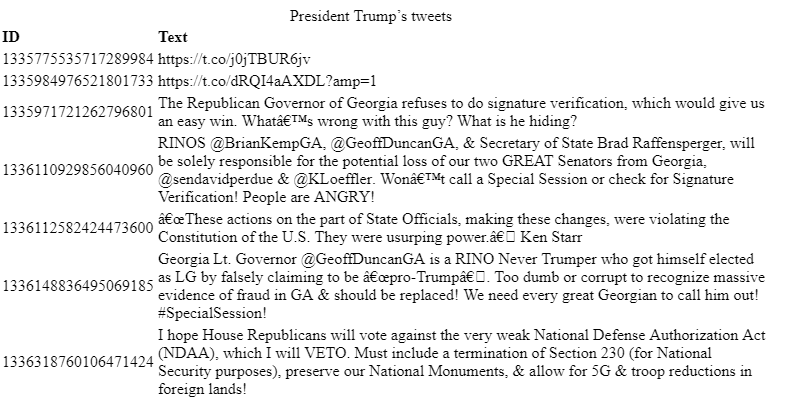
\includegraphics{final report resources/tweets.png}
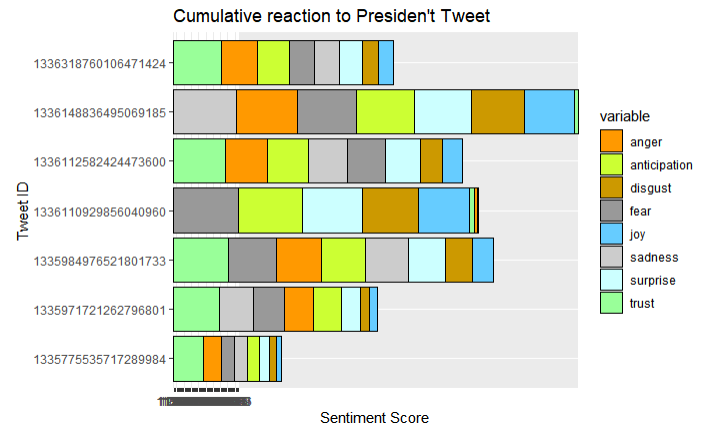
\includegraphics{final report resources/sentiments.png}

\hypertarget{cluster}{%
\paragraph{Cluster:}\label{cluster}}

Cluster centers through the reply thread have been consistent across
different tweets. These two denote two different kinds of replies but
doesn't necessarily indicate any political leanings. It seems that our
model classifies people or replies based on their emotiveness which can
be from either side of the fence. A further analysis of more clustering
might surface out more insights.

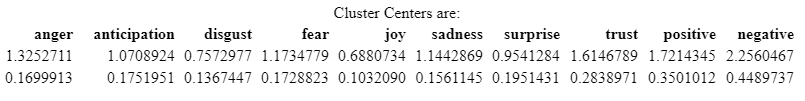
\includegraphics{final report resources/cluster center.png}
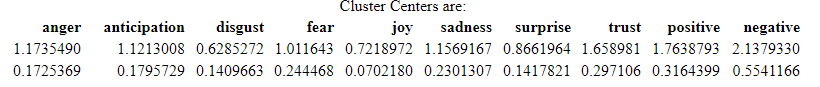
\includegraphics{final report resources/cluster center 2.png} My
clustering model shows similar distribution with all the replies in
these clusters. These down-sampled clusters show more higher density in
one which denoted our more poignant/ expressive responders and another
cluster which shows more withheld demeanour in replies.

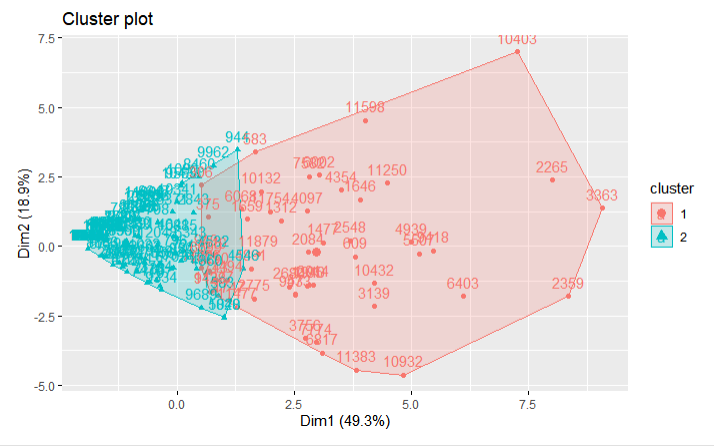
\includegraphics{final report resources/Cluster plot.png}
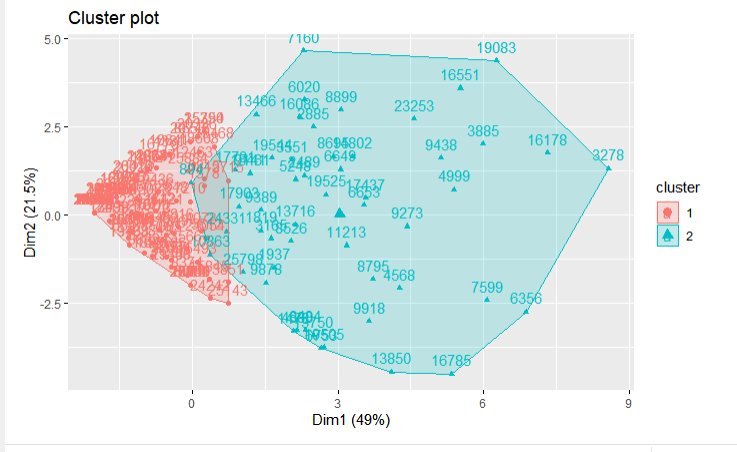
\includegraphics{final report resources/Cluster plot 2.png}

All clusters in every reply show a similar pattern of slightly more
negative emotions than positive.

\begin{figure}
\centering
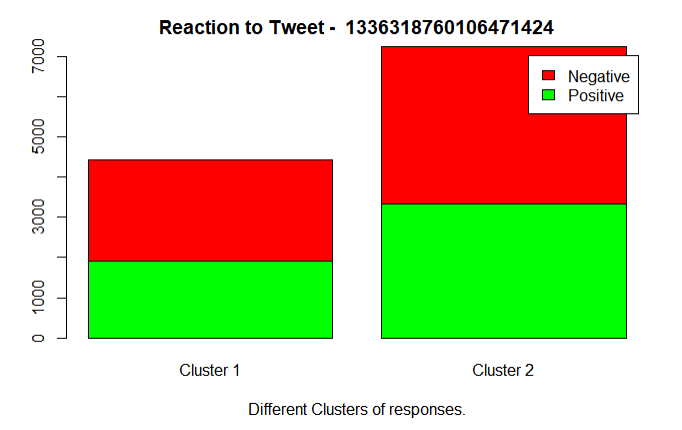
\includegraphics{final report resources/positivity.png}
\caption{Positivity within these clusters}
\end{figure}

\hypertarget{topics}{%
\paragraph{Topics:}\label{topics}}

Looking at the topic extracted from the tweets, it is quite conspicuous
that one of these Topic terms denote more Republican ideas and put more
weight over issues like Voter Fraud, court and Trump and other group
denote more democratic ideas as talk about issues like Covid and
country. 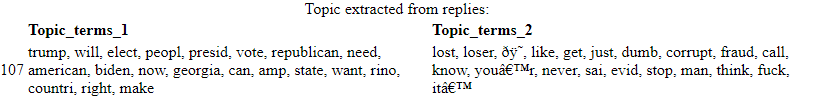
\includegraphics{final report resources/topics.png}

\begin{figure}
\centering
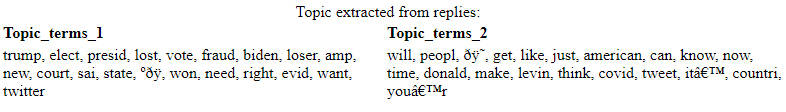
\includegraphics{final report resources/topics 2.png}
\caption{Topic terms example 2}
\end{figure}

\begin{figure}
\centering
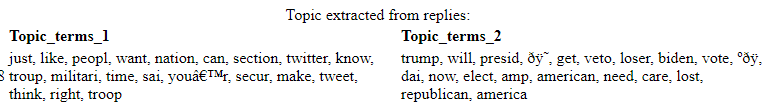
\includegraphics{final report resources/topics 3.png}
\caption{Topic terms example 3}
\end{figure}

Models developed in this study could be further enhanced to research on
the topic of social influences with different themes. Social feedback on
policies, presidents, and local government. We noticed overwhelming
negative sentiments, fear and distrust in masses along with factionism.
We need people who have more influence to more stringent checks and
higher standards.

\newpage

\newpage

\hypertarget{references}{%
\subsubsection{References}\label{references}}

\begingroup
\setlength{\parindent}{-0.5in}
\setlength{\leftskip}{0.5in}

\hypertarget{refs}{}
\begin{CSLReferences}{1}{0}
\leavevmode\hypertarget{ref-A__2016}{}%
A., Vishal, and S. S. Sonawane. 2016. {``Sentiment Analysis of Twitter
Data: A Survey of Techniques.''} \emph{International Journal of Computer
Applications} 139 (11): 5--15.
\url{https://doi.org/10.5120/ijca2016908625}.

\leavevmode\hypertarget{ref-inproceedings}{}%
Davidov, Dmitry, Oren Tsur, and Ari Rappoport. 2010. {``Enhanced
Sentiment Learning Using Twitter Hashtags and Smileys.''} In
\emph{Coling 2010 - 23rd International Conference on Computational
Linguistics, Proceedings of the Conference}, 2:241--49.

\leavevmode\hypertarget{ref-ge2018stock}{}%
Ge, Qi, Alexander Kurov, and Marketa Halova Wolfe. 2018. \emph{Stock
Market Reactions to Presidential Statements: Evidence from
Company-Specific Tweets}.

\leavevmode\hypertarget{ref-Keown2020survey}{}%
Keown, Callum. 2020. {``Here's How Much Trump's Tweets Are Influencing
Traders, Survey Reveals.''}
\url{https://www.marketwatch.com/story/heres-how-much-trumps-tweets-are-influencing-traders-survey-reveals-2020-01-16}.

\leavevmode\hypertarget{ref-kleczka2020effect}{}%
Kleczka, Justin. 2020. {``The Effect of President Trump's
Company-Specific Tweets on Company's Stocks.''}

\leavevmode\hypertarget{ref-Liu2019trump}{}%
Liu, Evie. 2020. {``Yes, Trump's Tweets Move the Stock Market. But Not
for Long.''}
\url{https://www.barrons.com/articles/donald-trump-twitter-stock-market-51567803655}.

\end{CSLReferences}

\endgroup

\bibliographystyle{unsrt}                 
\bibliography{r-references.bib}

\end{document}
